\documentclass{article}
\usepackage{amsmath, sfmath, multicol, tkz-euclide, array, enumerate, tcolorbox, tabularray}
\renewcommand{\familydefault}{\sfdefault}
\setlength{\parindent}{0cm}
\pagestyle{empty}
\usepackage[left=1in, top=0.5in, right=1in, bottom=0.5in]{geometry}
\tikzset{>=stealth}
\tcbset{colback=white}

\newcounter{example}[section]
\newenvironment{example}[1][]{\refstepcounter{example}\par\medskip
   {\color{red}\textbf{Example~\theexample. #1}}}{\medskip}

\begin{document}

\section*{Rotations}

\begin{tcolorbox}[colframe=orange!70!white, coltitle=black, title=\textbf{Today I Can}]
\begin{enumerate}
    \item Find images of rotated pre-images.
\end{enumerate}
\end{tcolorbox}
\bigskip

When a figure is rotated $90^\circ, \, 180^\circ, \text{ or } 270^\circ$ about the origin $O$ in a coordinate plane, you can use the following rules:

\begin{enumerate}
    \item Every $90^\circ$ rotated switches the $x$- and $y$-coordinates.    
    \item Every $90^\circ$ rotated is a new quadrant the point is in.
\end{enumerate}

\begin{center} 
\begin{tikzpicture}
	\draw[<->, >=stealth] (-2,0) -- (2,0);
	\draw[<->, >=stealth] (0,-2) -- (0,2);
	\node at (2,0) [anchor = west] {(+, 0)};
	\node at (0,2) [anchor = south] {(0, +)};
	\node at (-2,0) [anchor = east] {$(-, \, 0)$};
	\node at (0,-2) [anchor = north] {$(0, \, -)$};
	\node at (1,1) {(+, +)};
	\node at (-1,1) {$(-, \, +)$};
	\node at (-1,-1) {$(-, \, -)$};
	\node at (1,-1) {$(+, \, -)$};
\end{tikzpicture}
\end{center}

*** \emph{Unless otherwise stated, rotations are performed counterclockwise.} *** \newline\\

\begin{example}
Rotate each of the following. List the coordinates of the rotated image. \newline 

\begin{enumerate}[(a)]
    \item Rotate $90^\circ$ about the origin. \newline
    
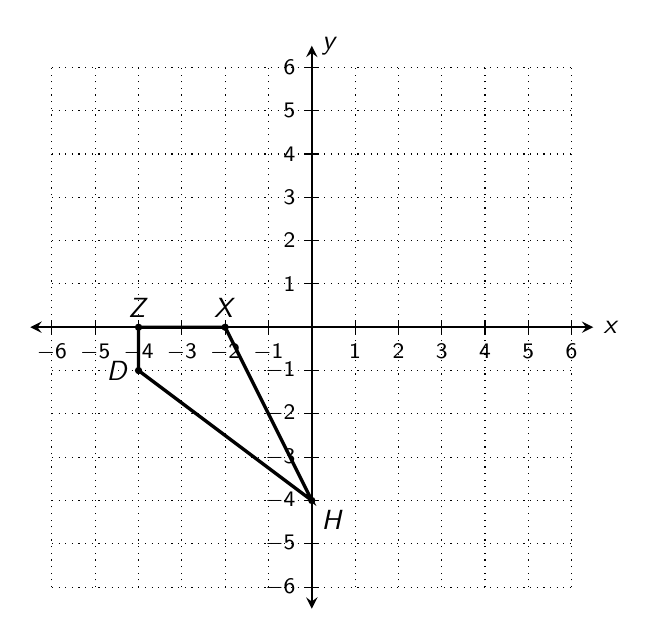
\begin{tikzpicture}[scale=0.55]
\draw[<->, thick] (-6.5,0) -- (6.5,0) node [right] {$x$};
\draw[<->, thick] (0,-6.5) -- (0,6.5) node [right] {$y$};
\draw[dotted] (-6,-6) grid (6,6);
\foreach \x in {-6,...,-1,,1,...,6}
\draw (\x, 0.15) -- (\x,-0.15) node [below] {\footnotesize $\x$};
\foreach \y in {-6,...,-1,,1,...,6}
\draw (0.15,\y) -- (-0.15,\y) node [left] {\footnotesize $\y$};
\coordinate (D) at (-4,-1);
\coordinate (Z) at (-4,0);
\coordinate (X) at (-2,0);
\coordinate (H) at (0,-4);
\draw[fill=black] (D) circle (2pt);
\draw[fill=black] (Z) circle (2pt);
\draw[fill=black] (X) circle (2pt);
\draw[fill=black] (H) circle (2pt);
\node at (D) [anchor = east] {$D$};
\node at (Z) [anchor = south] {$Z$};
\node at (X) [anchor = south] {$X$};
\node at (H) [anchor = north west] {$H$};
\draw[very thick] (D) -- (Z) -- (X) -- (H) -- cycle;
\end{tikzpicture}

\newpage 

\item Rotate $180^\circ$ about the origin. \newline 

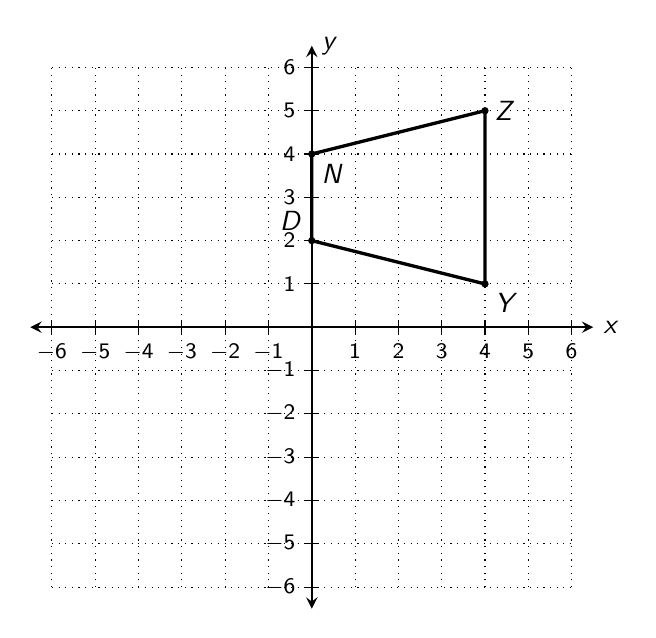
\begin{tikzpicture}[scale=0.55]
\draw[<->, thick] (-6.5,0) -- (6.5,0) node [right] {$x$};
\draw[<->, thick] (0,-6.5) -- (0,6.5) node [right] {$y$};
\draw[dotted] (-6,-6) grid (6,6);
\foreach \x in {-6,...,-1,,1,...,6}
\draw (\x, 0.15) -- (\x,-0.15) node [below] {\footnotesize $\x$};
\foreach \y in {-6,...,-1,,1,...,6}
\draw (0.15,\y) -- (-0.15,\y) node [left] {\footnotesize $\y$};
\coordinate (D) at (0,2);
\coordinate (Z) at (4,5);
\coordinate (N) at (0,4);
\coordinate (Y) at (4,1);
\draw[fill=black] (D) circle (2pt);
\draw[fill=black] (Z) circle (2pt);
\draw[fill=black] (N) circle (2pt);
\draw[fill=black] (Y) circle (2pt);
\node at (D) [anchor = south east] {$D$};
\node at (N) [anchor = north west] {$N$};
\node at (Z) [anchor = west] {$Z$};
\node at (Y) [anchor = north west] {$Y$};
\draw[very thick] (D) -- (N) -- (Z) -- (Y) -- cycle;
\end{tikzpicture}

\vspace{0.5in}

\item Rotate $270^\circ$ about the origin. \newline 

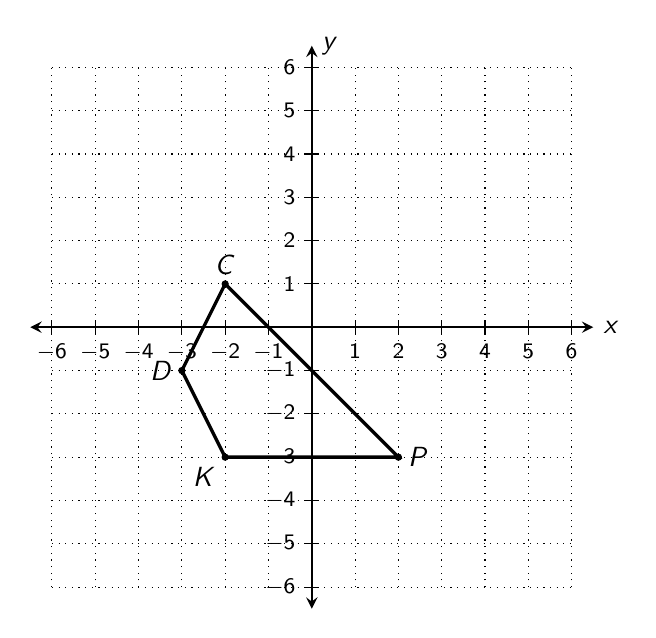
\begin{tikzpicture}[scale=0.55]
\draw[<->, thick] (-6.5,0) -- (6.5,0) node [right] {$x$};
\draw[<->, thick] (0,-6.5) -- (0,6.5) node [right] {$y$};
\draw[dotted] (-6,-6) grid (6,6);
\foreach \x in {-6,...,-1,,1,...,6}
\draw (\x, 0.15) -- (\x,-0.15) node [below] {\footnotesize $\x$};
\foreach \y in {-6,...,-1,,1,...,6}
\draw (0.15,\y) -- (-0.15,\y) node [left] {\footnotesize $\y$};
\coordinate (D) at (-3,-1);
\coordinate (C) at (-2,1);
\coordinate (P) at (2,-3);
\coordinate (K) at (-2,-3);
\draw[fill=black] (D) circle (2pt);
\draw[fill=black] (C) circle (2pt);
\draw[fill=black] (P) circle (2pt);
\draw[fill=black] (K) circle (2pt);
\node at (D) [anchor = east] {$D$};
\node at (C) [anchor = south] {$C$};
\node at (P) [anchor = west] {$P$};
\node at (K) [anchor = north east] {$K$};
\draw[very thick] (D) -- (C) -- (P) -- (K) -- cycle;
\end{tikzpicture}
\end{enumerate}
\end{example}

\end{document}
